\documentclass[ebook,10pt,oneside,openany]{memoir}
\usepackage[utf8x]{inputenc}
\usepackage[english]{babel}
\usepackage{url}

% for placeholder text
\usepackage{lipsum}
\usepackage{amsfonts, mathtools}
\usepackage[english]{babel}
\usepackage{amssymb, enumitem, enumerate, amsthm, amsmath, mathabx}

% ----- GRAPHICS/TIKZ-------
\usepackage{tikz, wrapfig, pgfplots}
\pgfplotsset{compat=1.14}
\usetikzlibrary{arrows,positioning,patterns,fadings}
%---------------------------


 % New commands
\newcommand{\naturals}{\mathbb{N}}
\newcommand{\reals}{\mathbb{R}}
\newcommand{\integers}{\mathbb{Z}}
\newcommand{\rationals}{\mathbb{Q}}
\newcommand{\complex}{\mathbb{C}}
\newcommand{\nullset}{\varnothing}
\newcommand{\diam}[1]{\mathrm{diam}\left(#1\right)}
\newcommand{\abs}[1]{\left\lvert#1\right\rvert}
\newcommand{\norm}[1]{\left\lVert#1\right\rVert}

\newcommand{\upRiemannint}[2]{
  \overline{\int_{#1}^{#2}}
}
\newcommand{\loRiemannint}[2]{
  \underline{\int_{#1}^{#2}}
}

% Renewed commands
\renewcommand{\iff}{\Leftrightarrow}
\renewcommand{\implies}{\Rightarrow}
\renewcommand{\bar}[1]{\widebar{#1}}


% My environments
\newtheorem*{theorem*}{Theorem}
\newtheorem{theorem}{Theorem}
\newtheorem{corollary}{Corollary}[theorem]
\newtheorem{lemma}[theorem]{Lemma}
\newtheorem{remark}{Remark}
\newtheorem{claim*}{Claim}
\newtheorem*{definition}{Definition}
% To ensure proper numbering of theorems within chapters
\numberwithin{theorem}{subsection} 


\title{My Notes on Real Analysis}
\author{Omanshu Thapliyal}

% To ensure equation numbering are correct for chapter 0
\renewcommand{\theequation}{\thechapter.\arabic{equation}}

\begin{document}
% To include Chapter Zero
\setcounter{chapter}{-1}
\maketitle


\tableofcontents

\chapter{Fundamentals}

If $A$ is a set and $x$ and element of the set, then $x\in A$, otherwise $x \notin A$. A set with no elements is denoted by $\nullset$, and a set $A$ is called nonempty if $A\neq \nullset$. If all elements of a set $A$ are also the elements of a set $B$, then $B$ \textit{contains} $A$, or $A \subset B$, therefore $A \subset A$ and $\nullset\in A$ hold trivially. We will often use this property to check for equality of two sets $A$ and $B$, i.e., $A=B \iff A\subset B$ and $B\subset A$.

\chapter{Constructing Reals}

Begin with the notion that we already know of the existence of natural numbers, denoted by $\naturals$ (let us skip Peano's axioms which formalize the existence of $\naturals$). Let us define the set of rational numbers $\rationals$ as $\rationals=\{\frac{m}{n}| m,n\in\naturals,n\neq 0\}$. Note that $\naturals[\rationals]$ are closed under addition and multiplication, i.e., if $a,b\in\naturals\Rightarrow a+b\in \naturals$. It can also be seen that $\naturals\in\rationals$ by definition.\\

The notion of sets is to be able to `collect' objects or elements into a `set', so to speak, so that we can perform set operations defined in Chapter 0. This provides us with a framework for constructing sets, comparing sets ($\subset, \subseteq$), and adding ($\cup$) sets together. However, the elements of the sets themselves are arbitrarily placed and have no order among them, i.e., if $A=\{a_0,a_1,a_2\}$, we can say that the element $a_1$ \textit{relates} to the set $A$ as $a_1\in A$, but we can not compare the individual elements of the set. In other words, the elements of the set so far are \textit{cardinal}, or, forming a set out of the elements is only assisting us to count them, but not \textit{order} them in any manner.\\

\section{Ordered Sets}

Consider the operation `$<$' on a set $S$ which is defined as follows:
\begin{enumerate}[label=\roman*.]
\item For some elements $x,y,z\in S$, if $x<y$ and $y<z$, then $x<z$.
\item If $x,y\in S$, then only one of the three can hold for the elements $x,y$, either $x<y$, or $x=y$ or $y<x$ (that is, $x$ either precedes, equals, or succeeds $y$).
This is called \textit{trichotomy}.\\
\textit{Note: }By trichotomy, the negation of `$<$' is `$\geq$'.
\end{enumerate}
The set $S$ together with the relation $<$ is called an \textit{ordered set}. Now that we have ordering in sets, we can talk define bounds, supremum and infimum of sets.\\

Consider a set $E\subset S$, where $S$ is an ordered set. If there exists $\beta\in S$ such that for every element $x\in E$, $x\leq \beta$, then the value $\beta$ bounds the set $E$ from above. Similarly we can define a lower bound $\beta$ for the set $E$ if $x\geq \beta$.
If the upper bound $\beta$ of $E$ satisfies the additional property that no smaller $\alpha < \beta$ exists in $S$, then $\beta$ is called the least upper bound, or $\beta = \sup{E}$. Similarly, $\alpha$ is called the infimum of $E$, $\alpha=\inf{E}$, if $\alpha$ is the greatest lower bound.\\

\begin{theorem}[Existence of supremum]
If set $E\subset S$ such that $E\neq \nullset$, and is bounded above, then $\alpha=\sup{E}$ exists in $S$. Further, if $L$ is the set of all upper bounds of $E$, then $\alpha=\inf{L}$.
\end{theorem}
The existence of supremum is essentially guaranteed for an ordered set if it is non-empty and bounded from above. In other words, if your nonempty set is bounded from above, I can always find the least upper bound. For instance, $E=\{\frac{1}{n}|n\in \naturals,n\neq0\}$. Clearly $E$ is contained in $\rationals$, which is an ordered set, and $1\in E$, so $E$ is nonempty. Further, $1$ is an upper bound for $E$, therefore, $\exists \sup{E}$. Also note that $0$ bounds $E$ from below, so $\exists \inf{E}$ as well.\\

This gives us a framework to compare elements of an ordered set, within the set, thereby forming ordinal sets. However, so far I can only tell if two elements precede, succeed, or equal each other. But we can perform other operations on these elements if we introduce the concept of \textit{fields}.

\section{Fields}
A field is a set $F$ with associated operations addition `$+$' and multiplication `$\times$' (these notes often omit the operator $\times$ to rewrite $a\times b$ as $ab$). The fields are \textit{closed} under both these operations, i.e., if $a,b\in F$, then the result of either operations $a\circ b \in F$. Axioms to define addition are:
\begin{enumerate}[label=A\arabic*.]
\item Closure: If $a,b\in F$, then $a+b\in F$
\item Commutativity: $a+b=b+a$
\item Associativity: $a+(b+c) = (a+b)+c$
\item Existence of identity: $\exists \,0\in F$ such that $x+0=x\,\forall x\in F$
\item Existence of inverse: $\exists -x\in F$ such that $x+(-x)=0\,\forall x\in F$
\end{enumerate}
Similarly, we can define multiplication using:
\begin{enumerate}[label=M\arabic*.]
\item Closure: If $a,b\in F$, then $ab\in F$
\item Commutativity: $ab=ba$
\item Associativity: $a(bc) = (ab)c$
\item Existence of identity: $\exists \,1\in F$ such that $x1=1x=x\,\forall x\in F$
\item Existence of inverse: $\exists 1/x\in F$ such that $x(1/x)=1\,\forall x\in F$
\end{enumerate}

\begin{remark}
Let us begin with the notion of $\naturals$. Now note that $\naturals$ is an ordered set. Now if we need to define an operation `$+$' that follows axioms A1-A5, we observe that $\naturals$ are incomplete. That is, if $\exists \,a\in\naturals$, then $\nexists -a\in \naturals$ such that they add up to the additive identity. In order to form a closed field under addition, we \textit{extend} $\naturals$ to $\integers$. This automatically means that $\naturals \subset \integers$, and $integers$ are closed under addition. now further notice that if we need to define a multiplication operation, $\integers$ are closed under it (i.e., M1. is satisfied), but once again $\nexists 1/x \in \integers, x\neq 0$ such that $x\cdot 1/x=1\,\forall x\in \integers$. This admits an automatic extension to the set $\mathbb{S}=\{\frac{1}{n}:n\in \integers \setminus \{0\} \}$. This forms a field $\mathbb{S}$ which satisfies M1-M5, but now does not satisfy A1 (consider $1/3, -1/4 \in\mathbb{S}$, but $1/3 + (-1/4)\notin \mathbb{S}$). This clearly demands and extension to a set $\rationals$ of the form $\naturals=\{\frac{p}{q}:p\in\integers,q\in \naturals \setminus \{0\}\}$. Thus, we get rational numbers if we start with the naturals.
\end{remark}

Note that an ordered set is not necessarily a field (example $\naturals$), and a field is not necessarily an ordered set (example $\mathbb{C}$, which will be seen later).

We can prove the following often used properties of addition and multiplication:
\begin{enumerate}[label=(a\arabic*)]
\item If $x+y=x+z$ then $y=z$ (from A3 and A4)
\item If $x+y=x$ then $y=0$ (from p1; also implies uniqueness of additive identity)
\item If $x+y=0$ then $y=-x$ (from p1 and A4; also implies uniqueness of additive inverse)
\item $-(-x)=x$ (apply A5 on $-x$)
\end{enumerate}
Very similarly,
\begin{enumerate}[label=(m\arabic*)]
\item If $x\neq0$, and $xy=yz$, then $y=z$
\item If $x\neq0$, and $xy=x$, then $y=1$
\item If $x\neq0$, and $xy=1$, then $y=1/x$
\item If $x\neq0$ then $1/(1/x)=x$
\end{enumerate}

\subsection{Ordered Fields}
If a field $F$ is an ordered field if it is also an ordered set and satisfies the following:
\begin{enumerate}[label=(OF\arabic*)]
\item $x+y<x+z$ if $x,y,z\in F$ and $y<z$
\item $xy>0$ if $x,y\in F,x>0$ and $y>0$
\end{enumerate}
A number is called \textit{positive} if $x>0$ and \textit{negative} if $x<0$.

\section{Constructing Reals}
It should be noted that the field $\rationals$ is incomplete. For example, $\exists p$ such that $p\cdot p=2$, but $p\in \rationals$. Consider Rudin's Example 1.1 which explains that if $A=\{p\in\rationals:p^2<2\}$ and $B=\{p\in\rationals:p^2>2\}$, then $A$ has no supremum in $\rationals$ and $B$ has no infimum in $\rationals$. In order to extend the least upper bound property in $\rationals$, we need to construct $\reals$.

\begin{theorem}[Real number field]
There exists an ordered field $\reals \supset \rationals$ such that $\reals$ has the least upper bound property.
\end{theorem}
\begin{proof}[Sketch of Proof]

\end{proof}

\begin{theorem}[Archimedean property]
If $x\in\reals, y\in\reals$ and $x>0$, then there exists a positive $n\in\naturals$ such that $nx>y$
\end{theorem}
\begin{corollary}
For every $x,y\in\reals$ and $x<y$, there exists some $p\in\rationals$ such that $x<p<y$.
\end{corollary}

\begin{theorem}
For every real $x>0$ and integer $n>0$ there exists a unique positive real $y$ such that $y^n=x$.
\end{theorem}
\begin{corollary}
If $a$ and $b$ are positive reals and $n\in\integers$, then $(ab)^{1/n} = a^{1/n}b^{1/n}$.
\end{corollary}

\section{Complex Field}
\begin{definition}
A complex number is an ordered pair  $(a,b)$ of real numbers $a,b$, i.e., $(a,b)\neq(b,a)$ if $a\neq b$.
\end{definition}
The set of such numbers is called $\complex$. Further defining the specific addition and multiplication for the field as:
\begin{definition}\label{complexOperators}
If $x,y\in\complex$ such that $x=(a,b),y=(c,d)$, then
\begin{equation*}
\begin{split}
x+y &= (a+c,b+d)\\
xy &= (ac-bd,ad+bc)
\end{split}    
\end{equation*}
\end{definition}

Try to prove A1-A5 and M1-M5 for the operations above in the field $\complex$.

Using these definitions, for any real number $x,y$ we have $(x,0)+(y,0)=(x+y,0)$, and $(x,0)(y,0)=(xy,0)$. This means that the multiplication and addition defined in Def. \ref{complexOperators} automatically satisfy the arithmetic of real number operations. Therefore, we constructed $\complex$ without defining $i^2=-1$, or extending $\reals$.\\
\begin{remark}
Note that we can easily prove using the definitions above that for some $i\coloneqq (0,1)$, $i\cdot i=-1$, and using that fact further prove that $(a,b)=a+bi$
\end{remark}



\chapter{Topology}

\section{Mapping}
So far we have seen how to construct sets, compare sets, and find `relations' between the elements of set. A natural extension are functional maps that take entire (sub)sets to different (sub)sets. A mapping, in this sense, is an abstract function which operates on sets by taking its individual elements to another set. This way, functional maps allow us to talk about comparisons of sets, relate sets, and to \textit{transform} one set to the other.

\begin{definition}
We define a \textbf{mapping} from a set $A$ to a set $B$ by any relation that takes the elements of $A$ to result in an element of $B$. It is denoted as $f:A\rightarrow B$ and for some $a\in A,a \mapsto f(a)$.
Suppose that $f$ maps a subset $E\subset A$ to a subset $V\subset B$.
Then we call the \textbf{image of $E$} under the \textbf{mapping $f$} as $f(E)=\{f(x)|x\in E\}\subset B$ and the \textbf{inverse image of $V$} as $f^{-1}(V)=\{x\in A|f(x)\in V\}\subset A$.
\end{definition}

\begin{enumerate}[label=D\arabic*.]
\item $f:A\rightarrow B$ is \textbf{onto/surjective} if $f(A)=B$. Or, if for any $y\in B \exists\,x\in A$ such that $y=f(x)$. $x_1,x_2\in A, x_1\neq x_2 \implies f(x_1) \neq f(x_2)$.
\item $f:A\rightarrow B$ is \textbf{one-to-one/injective} if $f^{-1}(y)$ is at most one point. Or, for any $y\in B \exists,$ at most one $x\in A$ such that $y=f(x)$. 
\item $f:A\rightarrow B$ is called \textbf{bijective} if it is both injective and surjective.
\end{enumerate}

\subsection{Cardinality}
We need the idea of cardinality so as to compare the sizes of sets. However, so far we have not restricted our sets to be `finite', or even defined what it is to be finite. But it should make sense to say that two sets $A$ and $B$ have the same number of elements, or \textit{cardinality}, if I can line them up in a train where one element of $A$ is next to the other element of $B$. At the end of this process, we know that $|A|=|B|$. Note that what we did was to find a bijection between the sets $A$ and $B$.
Therefore,
\begin{definition}
If $\exists$ a bijection $f$ between $A$ and $B$ such that $f:A\rightarrow B$, then the two sets have the same cardinality, or $A\sim B$.
\end{definition}
The symbol `$\sim$' is the equivalence relation and has the following properties:
\begin{enumerate}[label=(\alph*)]
\item Reflexive: $A\sim A$
\item Symmetric: $A\sim B\Rightarrow B\sim A$
\item Transitive: $A\sim B, B\sim C\Rightarrow A\sim C$
\end{enumerate}

\section{Finite Sets}
We denote the set of naturals by $\naturals=\{0,1,2,\cdots,n,\cdots\}$. Jet $J_n$ denote subsets of $\naturals$ as $J_1=\{1\}, J_2=\{1,2\},\cdots, J_n=\{1,2,\cdots,n\}$. In addition, we denote by $J_0=\nullset$ and $J=\naturals\setminus \{0\}$. These subsets of $\naturals$ allow us to find cardinality of other sets, provided we can find an equivalence (or, a bijection) between the set in question and some $J$.
\begin{definition}
A set $E$ is a \textbf{finite set} if $E\sim J_n$ for some $n\in \naturals$. Further, $n$ is defined to be the cardinality of the set $E$.\\
A set $F$ is considered \textbf{infinite} if it is not finite, or if $E\nsim J_n$ for any $n\in \naturals$.
\end{definition}

\subsection{Countable Sets}
$E$ is countable iff $E\sim J (=\naturals)$. \\
The word `countable' is an unfortunate usage of the English language, where it makes more sense to say \textit{listable}, because if I can create a list of the elements of $E$ as $\{e_1,e_2,\cdots,e_n,\cdots\}$, then $E$ is countable (listable, rather). 
Note that $\integers \sim \naturals$ as the elements of $\integers$ can be reordered to form a bijection with $\naturals$.\\
A useful corollary is the fact that \textbf{countable sets are infinite}. An unsurprising definition that follows up is $uncountable sets$ are sets that are `not countable'.

\subsubsection{Useful properties}
\begin{enumerate}[label=P\arabic*.]
\item Any infinite set contains a countable subset
\item Every infinite subset of countable sets is countable
\item \textit{Well-orderedness principle:} Every subset of $\naturals$ has a smallest element
\item \textit{Countable unions of countable sets are countable:} 
More formally,
\begin{enumerate}[label=P4.\arabic*]
    \item Let $A$ be a countable set and $E_\alpha,\alpha\in A$ be countable as well. Then $E=\bigcup\limits_{\alpha\in A} E_\alpha$ is countable.
    \item If $A$ is at most countable and so is $E_\alpha,\alpha\in A$, then $E=\bigcup\limits_{\alpha\in A} E_\alpha$ is at most countable.
\end{enumerate}
\end{enumerate}

From the above we can see that the set of rationals $\rationals\sim \naturals$. More generally, if $T^n$ denotes the set of all $n-$tuples such that each element in the tuple comes from a countable set, then $T$ is countable.

\section{Metric Spaces}
Consider a set $X$ with an added function $d:X\times X\rightarrow \reals$ or $(x,y)\mapsto d(x,y)$ for $\,x,y\in X, d(x,y)\in\reals$. Then the function $d$ is called a \textbf{distance} and the set with its associated distance a \textbf{metric space} if the following hold.
\begin{enumerate}[label=M\arabic*.]
\item $d(x,y) = 0\iff x=y$ (distance between two points is the same iff the points are the same)
\item $d(x,y)\geq 0$ (distance is non-negative)
\item $d(x,y)=d(y,x)$ (distance is non-directional)
\item $d(x,y)\leq d(y,z)+d(x,z)$ (taking detours is never better!)
\end{enumerate}

\subsection{Neighbourhoods}
Note that in context of a metric space, we have defined how far you are from a point $p$. This admits the definition of an  \textbf{$r-$neighbourhood} around point $p$, which is nothing but the set of points at most $r$ distance from $p$.

That is, $\mathcal{N}_r(p)\triangleq \{x\in X:d(p,x)<r\}$. Sometimes this is also called a ball of radius $r$ around point $p$, denoted by $B_r(p)$, as shown here.\\

% \begin{wrapfigure}{i}{0.35\textwidth}
\begin{center}
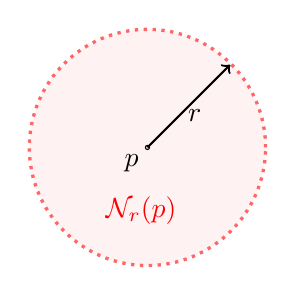
\begin{tikzpicture}
\filldraw[color=red!60, fill=red!5, very thick, dotted](0,0) circle (1.5);
\draw (0,0) circle [radius=0.75pt];
\draw [->, thick] (0,0) -- (1.05,1.05);
\draw (-0.2,-0.2) node {$p$};
\draw (0.6,0.4) node {$r$};
\draw (-0.08,-0.8) node [text=red] {$\mathcal{N}_r(p)$};
\end{tikzpicture}
\end{center}
% \end{wrapfigure}

Knowing the definition of a neighbourhood around a point, we can classify points based on these neighbourhoods as (for a point $p\in X$ and a subspace $E\subset X$):

\begin{enumerate}[label=D\arabic*.]
\item \textbf{Interior point:} $p\in X$ is an interior point of $E\subset X$ if $\exists\,r>0$ such that $\mathcal{N}_r(p)\subset E$.
\item \textbf{Limit point:} $p\in X$ is a limit point of set $E$ if \textit{every} neighbourhood of $p$ has a point $q\neq p$, i.e., $\left(\mathcal{N}_r(p)\setminus {p}\right) \cap E \neq \nullset$.
\item \textbf{Isolated point:} If $p\in E$ and $p$ is not a limit point, it is isolated.
\end{enumerate}

\subsection{Open \& Closed Sets}
We can also classify a set based on its constituent points as
\begin{enumerate}[label=S\arabic*.]
\item \textbf{Complement of a set:} If $E\subset X$, then its complement with respect to the metric space $X$ is $E^c=\{x\in X:x\notin E\}$
\item \textbf{Open set:} If all points of $E$ are interior points, it is an open set.
\item \textbf{Closed set:} If every limit point of $E$ is also a point in $E$, the set is closed
\item \textbf{Perfect set:} If $E$ is closed and every point of $E$ is a limit point, it is a perfect set.
\item \textbf{Bounded set:} If $\exists M\in \reals$ such that upon fixing $p\in E, d(p,x)<M\,\forall x\in E$, $E$ is bounded.
\item \textbf{Dense in $X$:}  If every $x\in X$ is a limit point of $E$, or a point of $E$ (or both), $E$ is dense in $X$.
\end{enumerate}

These definitions are abstractions of open intervals (open set), closed intervals (closed set), finite intervals (bounded set), `surfaces' of a set (closure), holes in an interval (isolated points), etc. These are very closely related to abstract intervals, to form continuums which are studied in topology. For instance, a limit point is closely related to sequences, as a limit point can be approximated by its neighbouring points.

Some properties of open and closed sets to be noted are:
\begin{enumerate}[label=(\roman*)]
\item $\nullset,X$ are open
\item If $E\subset X$ is open, then $E^c$ is closed.\\
This implies that $\nullset,X$ are both closed as well; finite sets are closed too because they have no limit points.
\item If $U,V\subset X$ are open sets, then $U \cup V$ is open.\\
Similarly, if $U,V\subset X$ are closed, then $U\cap V$ is closed (by (ii)).
\item More generally, if $\{U_\alpha\}_{\alpha\in A}$ are individually open $\forall \alpha\in A$, then $U=\bigcup\limits_{\alpha\in A} U_\alpha$ is open.\\
Using (ii), if $\{U_\alpha\}$'s are all closed for all $\alpha\in A$, $U=\bigcap\limits_{\alpha\in A} U_\alpha$ is closed.
\item $p$ is a limit point of $E$ iff $N_r(p)\cap E$ is infinite for any $r>0$.
\end{enumerate}

\begin{definition}
If $E\subset X$, then denote by $E'$ the set of all limit points of $E$, and by $\bar{E}=E\cup E'$. Then $\bar{E}$ is called the \textbf{closure} of $E$.
\end{definition}
The set $E$ is then closed iff $E=\bar{E}$ and clearly, $E\subset \bar{E}$, where the closure is a closed set. This means that the operation closure($\cdot$) on a set is idempotent, i.e., $\bar{E} = \overline{\bar{E}}$.
Also, for some $A_i\subset X$ for some $i=1,2,\cdots,n$ (finite), $\bar{\bigcup\limits^n_{i=1}A_i} = \bigcup\limits^n_{i=1}\bar{A_i}$, which can be proved by induction.

\section{Compact Sets}
A compact set abstracts the notion of mathematical infinities. Compact sets try to avoid infinities arising in two manners: a) infinite size of set (unboundedness), and b) infinities due to limit points not lying in the set (by making them `compact'). It is easier to understand what compactness means for a set by first defining a compact set, and then seeing relaxing which other properties makes a set non-compact.

\begin{definition}[Open Cover]
Consider a set $E\subset X$. If there exists a collection of open sets $G=\{G_\alpha\}$ such that $E\subset \bigcup\limits_{\alpha\in A}G_\alpha$, then $G$ is an open cover of $E$.
\end{definition}
\begin{definition}[Compact Set]
A set $E\subset X$ is compact if \textbf{every} open cover of $E$ has a finite subcover of $E$.
\end{definition}

So, if I have to prove a set is non-compact, I only need to find one counter example of an open cover of $E$ that does not contain a subcover of $E$.
On the other hand, to prove a set is compact is harder, because \textbf{every} open cover needs to have a finite subcover. For example, consider $E=\{1/n:n=1,2,\cdots\}$, is not compact. I can easily prove this by considering an open cover of the form $G_n=(1-1/n,1+1/n)$, which is a series of shrinking intervals centred around 1. But the limit point of $E$, which is $0$, never lies in a finite subcover.
Later on we will see that using Heine-Borel theorem requires this set to be closed in order to be compact, which it is not, since $0\notin E$.
On the other hand $E=\{1/n:n=1,2,\cdots\}\cup\{0\}$ is compact.

It is easier to understand what compactness means if we try to see how we can make a set non-compact. One obvious way to do so is by making the set so large that no finite subcover contains it. That is, \textit{make the set unbounded}. Consider a set $E=\{x\in \reals : x\geq0\}$. The infimum $0\in E$, but since the set is infinite in size, i.e., $\nexists M \in \reals$ such that $d(x,p)<M\,\forall x\in E$ for a fixed point $p$. This set is trivially noncompact. On the other hand, consider the set $E=(a,b)\subset\reals$. Despite the finite `size' of the interval (bounded trivially by $|b-a|$),the interval is not compact because it struggles with an infinity of the second kind.

\begin{center}
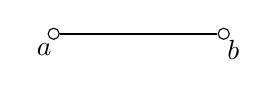
\begin{tikzpicture}
\draw (-0.08,0) circle [radius=2pt];
\draw (2.08,0) circle [radius=2pt];
\draw [thick] (0,0) -- (2,0);
\draw (-0.2,-0.2) node {$a$};bol
\draw (2.2,-0.2) node {$b$};
\end{tikzpicture}
\end{center}

This set has issues related to infinities of a different sort. No matter how close you approach to the limit point $a$ (or $b$), you never reach there, as it is not in your set. In fact, $(a,b)$ is topologically similar to $(-\infty,\infty)$! \\
An important thing to note, which is often confused, is that \textbf{every} open cover should have a finite subcover for a set to be compact. It is harder to prove compactness, and easier to prove noncompactness, as the latter requires one counter example of an open cover not having a finite subcover. Similarly, simply finding one open cover that has an open subcover leads to nothing. For instance, recall that the metric space $X$ is open (and also closed). So $X$ covers literally every subset of $X$! But that does not mean every subset of $X$ is compact, as compactness requires all open covers to have a finite subcover.\\

\begin{lemma}
\begin{enumerate}
\item Compact subsets of metric spaces are closed
\item Closed subsets of compact sets are compact
\end{enumerate}
\end{lemma}
\begin{corollary}
If $F$ is a closed set and $K\subset X$ a compact set, then $F\cap K$ is compact.
\end{corollary}

This also leads us naturally to the Heine-Borel Theorem. Recall from the discussion above that to make a set compact, we need to `fix' the two kinds of infinities we encountered. The first one is fixed by making our set small enough for there to be even a possibility of a finite (sub)cover, i.e., boundedness. The other fixes the existence of limit points, which introduce infinities around them, i.e., closed sets.

\begin{theorem}[Heine-Borel Theorem]
$K\subset \reals^k$ is compact $\iff K$ is closed and bounded. \textbf{note that this is only for Euclidean spaces}.
\begin{lemma}
Closed subsets of compact sets are compact.
\end{lemma}
\begin{lemma}
Closed $k-$cells in $reals^k$ are compact.
\end{lemma}
\end{theorem}

\begin{theorem}[Bolzano-Weierstrass Theorem]
Let $K\subset X$ be a compact set, and $E\subset K$ an infinite subset of $K$, them $E$ has a limit point in $K$.
\end{theorem}

\begin{theorem}[Kantor Intersection Theorem]
If $K_n\subset X$ is a sequence of nonempty compact sets such that $K_n\supset K_{n+1}$ for $n=1,2,\cdots$, then $\bigcap\limits_{i=1}^{\infty}K_i \neq \nullset$.
\end{theorem}

\subsection{Perfect Sets}
\begin{definition}
A nonempty set $P\subset X$ is a \textbf{perfect} set if $P$ is closed and all points $P$ are limit points of $P$, or if $P$ is closed and has no isolated points.
\end{definition}
\begin{theorem}[Perfect sets are uncountable]
If $P\subset \reals^k, P\neq \nullset$ is a perfect set, then $P$ is uncountable.
\end{theorem}

\subsection{Connected Sets} 
Two disjoint sets $A,B\subset X$  are \textbf{separated} if $\bar{A}\cap B\neq \nullset$ and ${A}\cap \bar{B}\neq \nullset$. We say that $E$ is \textbf{disconnected} if $\exists\, A,B$ such that $A,B\neq \nullset$, $A,B$ are separated, and $E=A\cup B$. Finally, a set $E\subset X$ is connected if it is not disconnected.\\
The concept of connectedness says that the set $E$ should not be breakable into two sets `far apart'. The notion of `far apart' is conveyed by the set being breakable into two open sets.

\begin{theorem}[Connected sets in $\reals$]
A set $E\subset \reals$ is connected iff it has the \textbf{interval property}: if $x,y\in E$, then $[x,y]\in E$ for some $x<y$.
\end{theorem}

\begin{lemma}
If $V\subset \reals$ is bounded above and $V\neq \nullset$, then $\sup{V}\in \bar{V}$.
\end{lemma}

\chapter{Sequences}

A \textbf{sequence} in $X$ is a mapping $f:\naturals\rightarrow X$. That is, a sequence is a list that is numbered.  The map is the relation between the entries of the list and number of the entry on the list.
We simply write $f(1)=p_1$ or $p_n=f(n)$ by omitting the map $f$ and only denoting the sequence by its terms.
We often misuse the notation to denote $\{p_n\}$ a sequence with terms $\{p_1,p_2,\cdots,p_n,\cdots\}$ which is the same notation as the elements $p_1,p_2,$etc., but the two are different.

\begin{definition}
We say a sequence $p_n$ converges to some $p\in X$ if for any $\varepsilon > 0,\,\exists N_\varepsilon\in \naturals $ such that $d(p_n,p)<\epsilon$ if $n\geq N_\varepsilon$.
\end{definition}
The definition of a convergent sequence is that it gets arbitrarily close to the term $p\in X$. This point $p$ is called the limit of the sequence. Note that this definition is equivalent to saying that $p_n$ is convergent if $p_n \in N_\varepsilon(p),\,\forall n\geq N_\varepsilon$. This clearly means that there are infinite points of the sequence which lie in $N_\varepsilon (p)$. Note that this property of a convergent sequence is often used to define infinite sets, neighbourhoods, open and closed sets. This is also the intuition behind the nomenclature of a `limit point', i.e., the limit point of the set has a sequence in the set whose limit is the point. 
Only finitely many points of a sequence $\{p_n\}$ lie outside any neighbourhood around the limit. Actually, we even know how many points would be outside, they would be points $\{p_1,p_2,\cdots,p_{N_\varepsilon}\}$.

\begin{remark}
\begin{enumerate}[label=R\arabic*.]
\item If a sequence $p_n\rightarrow p$, then the limit $p$ is unique.
\item If a sequence $p_n$ is convergent, then it is bounded.
\item Algebraic operations on Numeric Sequences: Consider two sequences $s_n\to s$ and $p_n\to p$,
\begin{enumerate}[label=R.2.\alph*]
    \item $\lim_{n\to\infty}(s_n+p_n) = s + p$
    \item $\lim_{n\to\infty}(cs_n) = cs$
    \item $\lim_{n\to\infty}(s_np_n) = sp$
    \item $\lim_{n\to\infty}(s_n/p_n) = s/p$ if $p\neq0$
\end{enumerate}
\end{enumerate}
\end{remark}

\subsection{Sequences in $\reals^k$}
Suppose $\{x_n\}_{n=1}^\infty\in\reals^k$ such that $x_n = \{x_{1,n},x_{2,n},\cdots,x_{k,n}\}\implies \{x_{i,n}\}$ is a sequence in $\reals$. These individual sequences are projections of the original sequence in $\reals^k$ in the form of components of $\{x_n\}$. Therefore, $\{x_n\}_{n=1}^\infty\in\reals^k,x_n\to a=\{a_1,a_2,\cdots,a_k\}$ if $x_{i,n}\to a_i$ for any $i=1,2,\cdots,k$.

\section{Subsequences}
Consider a sequence $\{p_n\}\in X$ and some indices $n_1,n_2,\cdots,n_k,\cdots\in \naturals$ such that they form an increasing sequence $n_1<n_2<\cdots<n_k<\cdots$, then we can use the new increasing ``sequence" of integers to index terms out of $p_n$. This newly drawn sequence of terms is a \textit{subsequence} denoted by $\{p_{n_k}\}_{k=1}^\infty$.

\begin{theorem}
If $\{p_n\}$ is a sequence in $X$ such that $p_n\to p$ as $n\to \infty$, then for any subsequence $\{p_{n_k}\}$, $p_{n_k}\to \infty$ as $k\to \infty$ as well.
\end{theorem}

\subsubsection{Sequences in a compact set}

\begin{enumerate}[label=(\roman*)]
\item Let $\{p_n\}$ be a sequence in a compact set $K\subset X$ then $\{p_n\}$ has a convergent subsequence.
\item {[Corollary of (i)]} If $\{p_n\}$ is a bounded sequence in $\reals^k$, then $\{p_n\}$ has a convergent subsequence. \textbf{(Bolzano-Weierstrass for Sequences)}
\end{enumerate}

\section{Subsequential Limits}
It often helps (how?) to look at a set of \textit{all} the subsequences of a sequence. This translates to the supremum and infimum values of the set of all the limits points of a sequence. Note that for a convergent sequence, this set should collapse to a single point. 
Let us denote the set of all limit points of the sequence by $E^*=\{p\in X : p_{n_k}\to p\}$ for some subsequence $\{p_{n_k}\}$, then the set $E^*$ is a closed set $\implies$ if $p$ is a limit point of $E^*$, then $p\in E^*$.\\

Note that this set need not even be countable, even though the set of values taken by the sequence itself is countably infinite. E.g., the sequence. $\{1/1,1/2,2/2,1/3,2/3,3/3,1/4,2/4,3/4,4/4,\cdots\}$ is forming the set of all rationals, but we can form subsequences out of it to converge to \textit{any} irrational number, so the set of susbequential limits for the sequence is actually infinite.

\section{Cauchy Sequences}
Cauchy sequences generalizes the idea of convergent sequences. Recall that a convergent sequence is one where all the points ($\forall n$) eventually ($\forall n \geq N_\varepsilon$) fall within an $\varepsilon$ radius neighbourhood ($N_\varepsilon(p)$) of the limit point $p$ ($\forall n\geq N_\varepsilon, p_n\in N_\varepsilon(p)$). This is a strict demand on the sequence $p_n$, and Cauchy sequences are slightly more tolerant of sequences that could not converge, but the terms of the sequence itself come arbitrarily close to each other.
\begin{definition}
\begin{enumerate}
\item {[Cauchy sequence.]} We say a sequence $\{p_n\}$ is Cauchy if for any $\varepsilon >0\,\exists N_\varepsilon$ such that $d(p_n,p_m)<\varepsilon\,\forall m,n\geq N_\varepsilon$.
\item {[Tail of a sequence.]} Let $E_N=\{p_N,p_{N+1},\cdots,p_{N+k},\cdots\}$, the $E_N$ is the ``tail" of the sequence $p_n$
\item {[Diameter of a set.]} For some metric subspace $E\subset X$, we define the diameter as the ``largest distance between any two points" in the set, i.e., $\diam{E}=\sup{\{d(p,q):p,q\in E\}}$
\end{enumerate}
\end{definition}
\noindent \textbf{Note:}\\
$\{p_n\}$ is Cauchy $\iff$ $\diam{E_n}\to 0$ as $n\to \infty \iff \diam{E_{N_\varepsilon}}\leq \varepsilon$, and Cauchy sequences are bounded.

Convergent sequence, in general, need us to know the limit $p$ apriori, in order to write the properties of the sequence. Cuachy sequence, since not necessarily convergent, do not need us to know the limit (which may or may not exist), and still comment upon the properties of the sequence. Furthermore, \textbf{if $p_n\to p, \implies\{p_n\}$ is Cauchy}. But Cauchy sequences are not necessarily convergent. E.g., let $p_n\in\rationals$ be such that $p_n\to \sqrt{2}$. Clearly, $p=\sqrt{2}\notin\rationals$, but $\{p_n\}$  is Cauchy in $\rationals$. In general, think of any sequence in $K\setminus\{p\}\subset X$ where $p$ is the limit of the sequence. The sequence remains Cauchy, but no longer converges in its set.

\begin{definition}
We call a metric space $X$ to be \textbf{complete} if every Cauchy sequence in $X$ is convergent.
\end{definition}

\begin{theorem}
\begin{enumerate}[label=(\roman*)]
\item If $X$ is a compact set, then $X$ is complete
\item {[Corollary]} $\reals^k$ is complete
\end{enumerate}
\end{theorem}
Therefore,
\begin{enumerate}[label=C\arabic*.]
\item Cauchy sequences in complete metric spaces are convergent ($\because$ in a complete metric all Cauchy sequences converge)
\item Compact metric spaces are complete
\item Euclidean spaces $\reals^k$ are compact, therefore complete
\item \textbf{$\implies$ Cauchy sequences in $\reals^k$ are convergent}.
\end{enumerate}

\subsection{Monotone Sequences}
In order to define monotonicity of sequences, we need an ordered subset of a metric space. The unsurprisingly banal definition of monotonicity that thus follows is that $\{p_n\}$ is monotonically increasing if $s_n\leq s_{n+1}\,\forall n\in \naturals$ and monotonically decreasing if $s_n \geq s_{n+1}\,\forall n\in\naturals$. Obviously, a sequence could monotonically increase (decrease) to (minus) infinity. If we have a way to bound the monotone sequence, it would be convergent. \\

Therefore, a monotone sequence $\{s_n\}$ is convergent $\iff$ $\{s_n\}$ is bounded. Further, we will use the following shorthand: $\{s_n\}\nearrow$ if $\{s_n\}$ is increasing, and $\{s_n\}\searrow$ if it is a decreasing sequence.

\section{Subsequential Limits, back to: $\limsup$ and $\liminf$}

The concept of subsequential limits is introduced so as to discuss the properties of all sequences, and not only convergent ones.
A subsequential limit is defined as the limit of a subsequence $s_{n_k}$ from the sequence $s_n$.
Collecting all such subsequential limts gives us a set $E=\{s:s_{n_k}\to s\, \text{ for all subsequences } s_{n_k} \text{ of } s_n\}$.
For convergent sequences, all subsequences have to converge to the same point, so the set $E$ collapses to a single point.
\subsection{Upper \& Lower limits of sequences}
For a sequence in $\reals$ we say:
\begin{itemize}
\item $s_n\to \infty$, if for any $M\in \reals\,\exists N_M\in\naturals$ such that $s_n>M\,\forall n\geq N_M$
\item $s_n\to -\infty$, if for any $M\in \reals\,\exists N_M\in\naturals$ such that $s_n<M\,\forall n\leq N_M$
\end{itemize}

Now consider sequences in the extended reals $\bar{\reals}=\reals\cup\{\infty,-\infty\}$.
Let us form a set of all subsequential limits same as above, but this time in $\bar{\reals}$. 
We define $\liminf$ and $\limsup$ for $E=\{x\in\bar{\reals}:s_n\to x\}$
\begin{itemize}
\item $s^*\triangleq \limsup\limits_{n\to\infty} {s_n}=\sup{E}\in \bar{\reals}$
\item $s_*\triangleq \liminf\limits_{n\to\infty} {s_n}=\inf{E}\in \bar{\reals}$
\end{itemize}

\subsection{Properties of $\limsup$}
Let $s^*=\limsup{s_n}=\sup{E}$, then
\begin{enumerate}[label=P(ls)\arabic*.]
\item There is a subsequence which converges to $s^*$, i.e., $s^*\in E\equiv\exists s_{n_k}\to s^*$
\item If $s^*<x$, then $\exists N$ such that $s_N < x\,\forall n\geq N$ or, there are finitely many $n$'s such that $s_n\geq x$
\item $s^*$ is unique
\item If $s_n\leq t_n\,\forall n\geq n_0$, then
\begin{enumerate}[label=(\roman*)]
    \item $\limsup{s_n}\leq \limsup{t_n}$
    \item $\liminf{s_n}\leq \liminf{t_n}$
\end{enumerate}
A particular case of above is if $s_n\leq M\,\forall n\geq n_0\implies \limsup{s_n}\leq M$
\end{enumerate}

\section{Series}
For a sequence $a_n$ in $\reals$, we can define a new sequence $s_n = \sum^n_{k=0} a_k$, i.e., the n-th term of a series is the n-th partial sum of a sequence.
This new sequence is called a \textit{series}.

Therefore, similar convergence criteria hold for a series as well.
For instance, the Cauchy criterion for series would be as follows.
$\sum^n_{k=0} a_k$ is convergent $\iff$ for any $\varepsilon>0\exists N_\varepsilon$ such that $\abs{\sum^m_{k=n} a_k}<\varepsilon$ for all $m,n>N_\varepsilon, m>n$.
\begin{definition}
We say $\sum a_n$ is \textit{absolutely convergent} if $\sum \abs{a_k}<\infty$.
\end{definition}
Absolute convergence is a stronger criterion and if a series $\sum a_n$ converges absolutely $\implies$ the series $\sum a_n$ converges.
Note that the converse need not be true, e.g, $s_n=\sum^n (-1)^n$.

\subsection{Convergence tests for series.}
\subsubsection{Comparison Test.}
Comparison test compares the given series in question with another series whose convergence (divergence) is known to us.
Suppose $\sum a_n$,$\sum c_n$ are two series and $c_n\geq  0$, then
\begin{enumerate}[label=(\alph*)]
    \item if $\abs{a_n}\leq c_n$ for all $n\geq n_0$ and the upper series converges $\sum c_n< \infty$, then $\sum a_n$ is convergent.
    \item if $\abs{a_n}\geq c_n$ for all $n\geq n_0$ and the upper series converges $\sum c_n = \infty$, then $\sum a_n$ is divergent.
\end{enumerate}

An interesting result for series convergence is the \textbf{Cauchy condensation test} which states that for an increasing, positive sequence $a_n$, such that $a_n\geq a_{n-1}\geq0, \forall n\geq 0$, $\sum a_n<\infty \iff \sum 2^k a_{2^k}< \infty$.
The intuition behind the condensation test is to split each partial sum and bound it by sums of terms as multiples of $2^k$. For instance, $s_7 = a_1+\cdots+a_7\leq a_1 + (a_2 + a_2) + (a_4+a_4+a_4+a_4)=a_1 + 2a_2 + 4a_4$, etc.

\subsubsection{Root and Ratio tests.}
\begin{theorem}[Root Test]
Let $_n\geq 0$ and let $\alpha = \limsup_{n\to\infty} \sqrt[\leftroot{-2}\uproot{2}n]{a_n}$, then
\begin{enumerate}[label=(\alph*)]
    \item if $\alpha < 1 \implies \sum a_n < \infty$.
    \item if $\alpha > 1 \implies \sum a_n = \infty$.
    \item if $\alpha = 1$, the root test is inconclusive.
\end{enumerate}
\end{theorem}

\begin{theorem}[Ratio Test]
For a series with terms $a_n\neq0$, 
\begin{enumerate}[label=(\alph*)]
    \item if $\limsup_{n\to\infty} \abs{\frac{a_{n+1}}{a_n}}< 1\implies \sum a_n < \infty$
    \item if $\abs{\frac{a_{n+1}}{a_n}} \geq 1\implies \sum a_n = \infty$
\end{enumerate}
\end{theorem}

\begin{remark}
Let $c_n>0$, then\\
$\liminf_{n\to \infty} \frac{c_{n+1}{c_n}} \leq \liminf_{n\to \infty} \sqrt[\leftroot{-2}\uproot{2}n]{c_n} \leq \limsup_{n\to \infty} \sqrt[\leftroot{-2}\uproot{2}n]{c_n} \leq \limsup_{n\to \infty} \frac{c_{n+1}}{c_n}$
\end{remark}
That is, the root test provides a tighter bound, but is numerically harder than the ratio test.
And if the ratio test is satisfied, root test is automatically satisfied as well.

\section{Power Series.}
For some $z\in \mathbb{C}$, we call the expression $\sum_{n=0}^\infty c_n z^n$ a power series.
Naturally, the convergence of $\sum c_n z^n$ depends on where $z$ lies in the complex plane.
We define by $R=\frac{1}{\alpha}$ the \textit{radius of convergence} of the power series $\sum c_n z^n$, where $\alpha = \limsup \sqrt[\leftroot{-2}\uproot{2}n]{\abs{c_n}}$.
\begin{theorem}
For $R=\frac{1}{\alpha}, R\in [0,\infty]$
\begin{enumerate}[label=(\roman*)]
    \item if $\abs{z}<R\implies \sum c_n z^n$ converges absolutely.
     \item if $\abs{z}>R\implies \sum c_n z^n$ diverges.
     \item if $\abs{z}>R$, the test is inconclusive.
\end{enumerate}
\end{theorem}



\chapter{Continuity of Functions}

\section{Limit of a function.}
Let $X$ and $Y$ be two metric spaces equipped with some distance metrics $d_X, d_Y$.
Let $E\subset Y$ and $f:E\to Y$, then we denote the \textit{limit of the function $f$} as it approaches the point $p\in X$ as $\lim_{x\to p}f(x)$ and define it as:
$f(x)\to q$ as $x\to p\equiv \lim_{x\to p} f(x)=q,$ if for any $\varepsilon>0\,\exists \delta_\varepsilon>0$ such that $d_Y(f(x),q) < \varepsilon$ if $0<d_X(x,p)<\delta_\varepsilon, x\in E$.
Note that speaking of the limit of a function at an isolated point (i.e., if $p\in E$ but $p\notin E'$) is irrelevant.
\begin{figure}[!ht]
    \centering
    \scalebox{.80}{% Pattern Info
 
\tikzset{
pattern size/.store in=\mcSize, 
pattern size = 5pt,
pattern thickness/.store in=\mcThickness, 
pattern thickness = 0.3pt,
pattern radius/.store in=\mcRadius, 
pattern radius = 1pt}
\makeatletter
\pgfutil@ifundefined{pgf@pattern@name@_bt4epe2mx}{
\pgfdeclarepatternformonly[\mcThickness,\mcSize]{_bt4epe2mx}
{\pgfqpoint{0pt}{0pt}}
{\pgfpoint{\mcSize+\mcThickness}{\mcSize+\mcThickness}}
{\pgfpoint{\mcSize}{\mcSize}}
{
\pgfsetcolor{\tikz@pattern@color}
\pgfsetlinewidth{\mcThickness}
\pgfpathmoveto{\pgfqpoint{0pt}{0pt}}
\pgfpathlineto{\pgfpoint{\mcSize+\mcThickness}{\mcSize+\mcThickness}}
\pgfusepath{stroke}
}}
\makeatother
\tikzset{every picture/.style={line width=0.75pt}} %set default line width to 0.75pt        

\begin{tikzpicture}[x=0.75pt,y=0.75pt,yscale=-1,xscale=1]
%uncomment if require: \path (0,300); %set diagram left start at 0, and has height of 300

%Shape: Polygon Curved [id:ds7313279635399221] 
\draw   (96,85) .. controls (97,64) and (230,52) .. (230,70) .. controls (230,88) and (194,71) .. (214,101) .. controls (234,131) and (175,149) .. (155,119) .. controls (135,89) and (95,106) .. (96,85) -- cycle ;
%Shape: Ellipse [id:dp9151376985030744] 
\draw  [pattern=_bt4epe2mx,pattern size=6pt,pattern thickness=0.75pt,pattern radius=0pt, pattern color={rgb, 255:red, 128; green, 128; blue, 128}] (142.28,81.2) .. controls (146.96,71.19) and (164.94,69.7) .. (182.46,77.88) .. controls (199.97,86.05) and (210.39,100.79) .. (205.72,110.8) .. controls (201.04,120.81) and (183.06,122.3) .. (165.54,114.12) .. controls (148.03,105.95) and (137.61,91.21) .. (142.28,81.2) -- cycle ;
%Shape: Polygon Curved [id:ds132327224769744] 
\draw   (281,58) .. controls (301,48) and (289,25) .. (340,32) .. controls (391,39) and (351,88) .. (371,118) .. controls (391,148) and (334,146) .. (314,116) .. controls (294,86) and (261,68) .. (281,58) -- cycle ;
%Curve Lines [id:da8275404505595068] 
\draw [color={rgb, 255:red, 0; green, 0; blue, 0 }  ,draw opacity=1 ] [dash pattern={on 0.84pt off 2.51pt}]  (201,117) .. controls (259.12,92.37) and (303.65,137.61) .. (346.54,139.92) ;
\draw [shift={(348.5,140)}, rotate = 181.32] [color={rgb, 255:red, 0; green, 0; blue, 0 }  ,draw opacity=1 ][line width=0.75]    (10.93,-3.29) .. controls (6.95,-1.4) and (3.31,-0.3) .. (0,0) .. controls (3.31,0.3) and (6.95,1.4) .. (10.93,3.29)   ;

%Curve Lines [id:da9060207894942087] 
\draw [color={rgb, 255:red, 0; green, 0; blue, 0 }  ,draw opacity=1 ] [dash pattern={on 0.84pt off 2.51pt}]  (148,75) .. controls (206.71,50.12) and (249.57,27.23) .. (316,30.94) ;
\draw [shift={(317,31)}, rotate = 183.42] [color={rgb, 255:red, 0; green, 0; blue, 0 }  ,draw opacity=1 ][line width=0.75]    (10.93,-3.29) .. controls (6.95,-1.4) and (3.31,-0.3) .. (0,0) .. controls (3.31,0.3) and (6.95,1.4) .. (10.93,3.29)   ;

%Shape: Circle [id:dp3248341251389637] 
\draw   (143.8,87.78) .. controls (143.66,80.75) and (149.24,75.06) .. (156.27,75.06) .. controls (163.29,75.06) and (169.1,80.75) .. (169.24,87.78) .. controls (169.39,94.8) and (163.8,100.5) .. (156.78,100.5) .. controls (149.75,100.5) and (143.94,94.8) .. (143.8,87.78) -- cycle ;
%Shape: Circle [id:dp6767491936815082] 
\draw   (297.92,67.28) .. controls (297.72,56.94) and (305.93,48.56) .. (316.27,48.56) .. controls (326.61,48.56) and (335.16,56.94) .. (335.37,67.28) .. controls (335.57,77.62) and (327.36,86) .. (317.02,86) .. controls (306.68,86) and (298.13,77.62) .. (297.92,67.28) -- cycle ;
%Curve Lines [id:da5288665296815309] 
\draw [color={rgb, 255:red, 0; green, 0; blue, 0 }  ,draw opacity=1 ]   (168,95) .. controls (227,70) and (244.5,81.5) .. (311.5,85.5) ;


%Curve Lines [id:da027014413608954735] 
\draw [color={rgb, 255:red, 0; green, 0; blue, 0 }  ,draw opacity=1 ]   (151.5,75.5) .. controls (210.5,50.5) and (249.27,44.56) .. (316.27,48.56) ;



% Text Node
\draw (131,84) node   {$E$};
% Text Node
\draw (143,135) node   {$X$};
% Text Node
\draw (392.5,132.5) node   {$Y$};
% Text Node
\draw (157.5,83.5) node   {$p$};
% Text Node
\draw (184,106) node   {$\mathcal{N}_{{\delta }_{\varepsilon }}( p)$};
% Text Node
\draw (318.5,63) node   {$q$};
% Text Node
\draw (332.5,91.5) node   {$\mathcal{N}_{\varepsilon }( q)$};
% Text Node
\draw (253,119) node   {$f:E\rightarrow X$};


\end{tikzpicture}}
    \caption{Pictorial mapping of neighbourhood of $p\in E$ to $q\in Y$ under $f$}
    \label{fig:contNeigh}
\end{figure}

This definition is represented in Fig. \ref{fig:contNeigh} where $\mathcal{N}_{\delta_\varepsilon}(p)$ gets mapped to $\mathcal{N}_\varepsilon (q)$.
Since $\varepsilon$ is arbitrary, the neighbourhood around point $q$ can be made arbitrarily small, and still one would be able to find a corresponding point $x$ in the $\delta_\varepsilon$ neighbourhood of $p$.
Note that there could be a hole in the neighbourhood $\mathcal{N}_{\varepsilon}$ at $f(p)$.
That is, for the definition of the limit $\lim_{x\to p} f(x)$, the value of the function at $p$ is irrelevant.

An alternate \textit{sequential definition} of the limit of a function at a point uses the preservation of sequential limits under functional mappings.
For any sequence $p_n$ in $E$, if $p_n\to p, p_n\neq p$ holds then $f(p_n)\to q$ $\iff \lim_{x\to p}f(x)=q$.
Note that similar definitions of limit hold for functions in higher dimensions.
That is, $\lim_{x\to p}f(x)=q=(q_1,\cdots,q_k) \iff \lim_{x\to p}f_i(x)=q_i$ for $i=1,2,\cdots,k$.

The sequential definition of limits of a function is very useful since it helps us to borrow the important results of sequence convergence algebra, and use them to automatically get limit algebra results.
These limit algebra results are as follows.
If $\lim_{x\to p}f(x)$, $\lim_{x\to p}g(x)$ exist, then
\begin{enumerate}[label=(\roman*)]
    \item  $\lim_{x\to p}\alpha f(x) + \beta g(x) = \alpha \lim_{x\to p}f(x) + \beta \lim_{x\to p} g(x)$
    \item $\lim_{x\to p} f(x)\cdot g(x) = \lim_{x\to p}f(x)\cdot \lim_{x\to p}g(x)$
    \item $\lim_{x\to p} \dfrac{f(x)}{g(x)} = \dfrac{\lim_{x\to p}f(x)}{\lim_{x\to p}g(x)}$\\
    provided $\lim_{x\to p}g(x)\neq 0$ and $g(x)\neq 0$.
\end{enumerate}

\subsection{Limits at infinity.}
Recall that $\bar{\reals}=\reals\cup\{-\infty,+\infty\}$. We can define neighbourhoods in $\bar{\reals}$ as $(x-r,x+r)$ if $x\in\reals, (a,+\infty)$ when $x=+\infty$, and $(-\infty,b)$ when $x=-\infty$ ($a,b\in\reals$).
If $E\subset\reals$, then $+\infty$ is a limit point of $E$ iff $E$ is unbounded above, and $-\infty$ is a limit point if $E$ iff $E$ is unbounded below.
Now if $+\infty\in E',f:E\to\reals,$ we can talk about $\lim_{x\to\infty}f(x)=L\in\reals\iff \abs{f(x)-L}<\varepsilon$ if $x>a_\varepsilon,x\in E,\lim_{x\to a}f(x)=+\infty$ if $a\in E'$.

However, one has to be aware of indeterminate forms such as $\infty-\infty,0\cdot(\pm\infty),\pm\infty/\pm\infty$ when applying algebraic properties to limits.

\section{Continuity of a function.}
Using the definition of limits of a function, we can now define what it means for a function to be continuous at a point.
A function $f:E\to Y$ is continuous at a point $p$ if for any $\varepsilon>0$, $\exists \delta\varepsilon >0$ such that $d_Y(f(x),f(p))< \varepsilon$ if $d_X(x,p)<\delta_\varepsilon$ and $x\in E$.
Or, $f\left(\mathcal{N}_{\delta_\varepsilon}(p)\cap E\right) \subset \mathcal{N}_\varepsilon(f(p))$.
Comparing this with the definition of a limit, we find one key difference.
For the definition of a limit, the point $p\in E'$ is a limit point.

This has two consequences.
For some $f:E\to Y$ and $p\in E$
\begin{enumerate}
\item If $p\in E'$ then if $f$ is continuous at $p \iff \lim{x\to p} f(x) = f(p)$
\item If $p\notin E'$, or $p$ is an isolated point, then \textbf{any} function is continuous at $p$
\end{enumerate}

\subsection{Continuity of Compositions.}
Suppose $a\in A\subset X, b\in B\subset Y$.
Further suppose $f:A\to Y, f(A)\subset B$ and $g:B\to Z$.
If we define $g\circ f (x)=g(f(x)), x\in A$, then $g\circ f:A\to Z$, then the continuity of $f$ at $a$ and $g$ at $f(x)$ implies the continuity of $g\circ f$ at $a$.
This is a consequence of the sequential characterization of continuity.

\subsection{Global Continuity Theorem.}
Global continuity theorem states that for continuous functions, the pre-image of any open (closed) set is open (closed) [see Fig. \ref{fig:gct}].
\begin{theorem}[Global Continuity Theorem.]
A function $f:E\to Y$ is continuous $\iff$ for \emph{any} open set $V\subset Y, f^{-1}(V)$ is also open.
\end{theorem}
As a consequence, the pre-image of a closed set is also closed under continuous functions since if $V (f^{-1}(V))$  is open, $V^c (f^{-1}(V^c) = f^{-1}(V^c)^c)$ is closed.
\begin{figure}[!ht]
    \centering
    \scalebox{0.80}{


\tikzset{every picture/.style={line width=0.75pt}} %set default line width to 0.75pt        

\begin{tikzpicture}[x=0.75pt,y=0.75pt,yscale=-1,xscale=1]
%uncomment if require: \path (0,488); %set diagram left start at 0, and has height of 488

%Shape: Polygon Curved [id:ds026328184733499738] 
\draw   (94,238) .. controls (114,228) and (204,218) .. (184,238) .. controls (164,258) and (164,268) .. (184,298) .. controls (204,328) and (80,339) .. (94,298) .. controls (108,257) and (74,248) .. (94,238) -- cycle ;
%Shape: Polygon Curved [id:ds5677540075211358] 
\draw   (263,252) .. controls (283,242) and (334,158) .. (353,252) .. controls (372,346) and (349,308) .. (313,332) .. controls (277,356) and (299,335) .. (279,305) .. controls (259,275) and (243,262) .. (263,252) -- cycle ;
%Shape: Circle [id:dp6087537463141861] 
\draw  [dash pattern={on 4.5pt off 4.5pt}] (114,280) .. controls (114,267.85) and (123.85,258) .. (136,258) .. controls (148.15,258) and (158,267.85) .. (158,280) .. controls (158,292.15) and (148.15,302) .. (136,302) .. controls (123.85,302) and (114,292.15) .. (114,280) -- cycle ;
%Shape: Circle [id:dp5294184080370192] 
\draw  [dash pattern={on 4.5pt off 4.5pt}] (271,271.5) .. controls (271,249.68) and (288.68,232) .. (310.5,232) .. controls (332.32,232) and (350,249.68) .. (350,271.5) .. controls (350,293.32) and (332.32,311) .. (310.5,311) .. controls (288.68,311) and (271,293.32) .. (271,271.5) -- cycle ;
%Curve Lines [id:da8515105365836626] 
\draw [color={rgb, 255:red, 0; green, 0; blue, 0 }  ,draw opacity=1 ] [dash pattern={on 0.84pt off 2.51pt}]  (136,258) .. controls (195,233) and (267,231) .. (310.5,232) ;


%Curve Lines [id:da8016838777386179] 
\draw [color={rgb, 255:red, 0; green, 0; blue, 0 }  ,draw opacity=1 ] [dash pattern={on 0.84pt off 2.51pt}]  (136,302) .. controls (195,277) and (276.5,311) .. (320,312) ;



% Text Node
\draw (150,350) node   {$X$};
% Text Node
\draw (295.5,350.5) node   {$Y$};
% Text Node
\draw (321,222) node   {$V$};
% Text Node
\draw (119,248) node   {$f^{-1}( V)$};


\end{tikzpicture}}
    \caption{Pre-image of an open set under a continuous function}
    \label{fig:gct}
\end{figure}

\section{Compactness and Continuity.}
Compactness is preserved by continuous functions.
That is, if $X$ is  compact metric space and $f:X\to Y$ is continuous, then $f(X)$ is also compact.
This is a consequence of global continuity theorem applied to the definition of compactness (finite open sub-cover for any cover of the set $f(X)$).

\subsection{Continuity of inverse.}
If $X$ is compact and $f:X\to Y$ continuous and invertible, then its inverse $f^{-1}:Y\to X$ is also continuous.

The continuity of inverse functions can fail for non-compact sets.
For example, $f:[0,2\pi)\to\reals^2$ be defines as $f(t) = (\cos{t},\sin{t})$.
The continuity of this function breaks at $(1,0)\in\reals^2$.
$f^{-1}(1,0)=0$, and $\left(\cos{1/n},-\sin{1/n}\right)\to (1,0)$ as $n\to\infty$, but, $f^{-1}\left(\cos{\frac{1}{n}},-\sin{\frac{1}{n}}\right)= 2\pi-\frac{1}{n}=2\pi$. 

\subsection{Euclidean spaces and continuity.}
If $X$ is compact and $f:X\to \reals^k$, then $f$ is bounded.
That is, $\exists M>0$ such that $\abs{f(x)}\leq M\,\forall x\in X$.
\begin{remark}
A special case arises when $f$ maps to $reals$, i.e., $f:X\to \reals$.
If $f$ is continuous and $X$ compact, then $\sup$ and $\inf$ of $f$ are attained in $X$.
That is, $\exists x^*,x_*\in X$ such that $f(x_*)=\inf_{x\in X}f(x)=m$ and $f(x^*)=\sup_{x\in X}f(x)=M$. 
\end{remark}

\section{Uniform Continuity.}
Uniform continuity is a stronger notion which says that the neighbourhood of radius $\delta_\varepsilon$ around a point $x$ gets mapped to a neighbourhood of radius $\varepsilon$.
Further, there exists $\delta_\varepsilon$ such that the \emph{same} $\delta_\varepsilon$ works for all points $x\in X$.

That is, for any $\varepsilon>0,\,\exists \delta_\varepsilon>0$ such that $d_Y(f(p),f(x))<\varepsilon$ if $d_X(p,x)<\delta_\varepsilon$ for \emph{any} $x\in X$.
\begin{theorem}
If $X$ is compact, $f:X\to Y$ continuous $\implies f:X\to Y$ is uniformly continuous.
\end{theorem}

\section{Continuity and Connectedness.}
Continuity preserves connctedness.
Suppose $f:X\to Y$ is continuous  and $E\subset X$ is connected, then $f(E)\subset Y$ is connected as well.

This is not hard to visualize as shown in Fig. \ref{fig:contConnect}.
Suppose the image $f(E)$ of a connected set $E$ is disconnected.
This would result in a contradiction of $f$ being discontinuous since there would be some points for which the pre-image of some $\varepsilon$ neighbourhood does not lie in the connected set $E$.
The only way $f$ would be continuous, is for $E$ to be disconnected too!
This contradicts with the assumption that $E$ is connected.
\begin{figure}[!ht]
    \centering
    \scalebox{0.75}{


% Pattern Info
 
\tikzset{
pattern size/.store in=\mcSize, 
pattern size = 5pt,
pattern thickness/.store in=\mcThickness, 
pattern thickness = 0.3pt,
pattern radius/.store in=\mcRadius, 
pattern radius = 1pt}
\makeatletter
\pgfutil@ifundefined{pgf@pattern@name@_3ey3x60w6}{
\pgfdeclarepatternformonly[\mcThickness,\mcSize]{_3ey3x60w6}
{\pgfqpoint{0pt}{-\mcThickness}}
{\pgfpoint{\mcSize}{\mcSize}}
{\pgfpoint{\mcSize}{\mcSize}}
{
\pgfsetcolor{\tikz@pattern@color}
\pgfsetlinewidth{\mcThickness}
\pgfpathmoveto{\pgfqpoint{0pt}{\mcSize}}
\pgfpathlineto{\pgfpoint{\mcSize+\mcThickness}{-\mcThickness}}
\pgfusepath{stroke}
}}
\makeatother

% Pattern Info
 
\tikzset{
pattern size/.store in=\mcSize, 
pattern size = 5pt,
pattern thickness/.store in=\mcThickness, 
pattern thickness = 0.3pt,
pattern radius/.store in=\mcRadius, 
pattern radius = 1pt}
\makeatletter
\pgfutil@ifundefined{pgf@pattern@name@_qsk0qv6vp}{
\pgfdeclarepatternformonly[\mcThickness,\mcSize]{_qsk0qv6vp}
{\pgfqpoint{0pt}{-\mcThickness}}
{\pgfpoint{\mcSize}{\mcSize}}
{\pgfpoint{\mcSize}{\mcSize}}
{
\pgfsetcolor{\tikz@pattern@color}
\pgfsetlinewidth{\mcThickness}
\pgfpathmoveto{\pgfqpoint{0pt}{\mcSize}}
\pgfpathlineto{\pgfpoint{\mcSize+\mcThickness}{-\mcThickness}}
\pgfusepath{stroke}
}}
\makeatother

% Pattern Info
 
\tikzset{
pattern size/.store in=\mcSize, 
pattern size = 5pt,
pattern thickness/.store in=\mcThickness, 
pattern thickness = 0.3pt,
pattern radius/.store in=\mcRadius, 
pattern radius = 1pt}
\makeatletter
\pgfutil@ifundefined{pgf@pattern@name@_2eh8co567}{
\pgfdeclarepatternformonly[\mcThickness,\mcSize]{_2eh8co567}
{\pgfqpoint{0pt}{-\mcThickness}}
{\pgfpoint{\mcSize}{\mcSize}}
{\pgfpoint{\mcSize}{\mcSize}}
{
\pgfsetcolor{\tikz@pattern@color}
\pgfsetlinewidth{\mcThickness}
\pgfpathmoveto{\pgfqpoint{0pt}{\mcSize}}
\pgfpathlineto{\pgfpoint{\mcSize+\mcThickness}{-\mcThickness}}
\pgfusepath{stroke}
}}
\makeatother
\tikzset{every picture/.style={line width=0.75pt}} %set default line width to 0.75pt        

\begin{tikzpicture}[x=0.75pt,y=0.75pt,yscale=-1,xscale=1]
%uncomment if require: \path (0,488); %set diagram left start at 0, and has height of 488

%Shape: Polygon Curved [id:ds6161245015316863] 
\draw   (91,324) .. controls (111,314) and (129,335) .. (140,366) .. controls (151,397) and (116,408) .. (106,461) .. controls (96,514) and (82,418) .. (32,426) .. controls (-18,434) and (71,334) .. (91,324) -- cycle ;
%Shape: Polygon Curved [id:ds5849125845389338] 
\draw   (241,332) .. controls (243,286) and (317,368) .. (290,374) .. controls (263,380) and (301,429) .. (256,469) .. controls (211,509) and (243,449) .. (214,433) .. controls (185,417) and (239,378) .. (241,332) -- cycle ;
%Shape: Polygon Curved [id:ds4782088463335614] 
\draw   (421,335) .. controls (423,289) and (497,371) .. (470,377) .. controls (443,383) and (481,432) .. (436,472) .. controls (391,512) and (423,452) .. (394,436) .. controls (365,420) and (419,381) .. (421,335) -- cycle ;
%Snip Round Single Corner Rect [id:dp8600539012008661] 
\draw  [pattern=_3ey3x60w6,pattern size=6pt,pattern thickness=0.75pt,pattern radius=0pt, pattern color={rgb, 255:red, 0; green, 0; blue, 0}] (252.41,357.43) .. controls (262,352.17) and (270.56,356.02) .. (271.53,366.02) -- (276.11,413.25) -- (260.51,440.88) -- (243.15,450.4) -- (235.05,366.95) -- cycle ;
%Snip Round Single Corner Rect [id:dp31583524424949627] 
\draw  [pattern=_qsk0qv6vp,pattern size=6pt,pattern thickness=0.75pt,pattern radius=0pt, pattern color={rgb, 255:red, 0; green, 0; blue, 0}] (433.41,359.43) .. controls (443,354.17) and (451.56,358.02) .. (452.53,368.02) -- (457.11,415.25) -- (441.51,442.88) -- (424.15,452.4) -- (416.05,368.95) -- cycle ;
%Left Arrow [id:dp7160761384205165] 
\draw  [dash pattern={on 4.5pt off 4.5pt}] (382,391) -- (350.8,371) -- (350.8,381) -- (304,381) -- (304,401) -- (350.8,401) -- (350.8,411) -- cycle ;
%Shape: Polygon Curved [id:ds5344624629491945] 
\draw  [pattern=_2eh8co567,pattern size=6pt,pattern thickness=0.75pt,pattern radius=0pt, pattern color={rgb, 255:red, 0; green, 0; blue, 0}] (67,361) .. controls (87,351) and (138,359) .. (118,379) .. controls (98,399) and (83,374) .. (103,404) .. controls (123,434) and (87,451) .. (67,421) .. controls (47,391) and (47,371) .. (67,361) -- cycle ;
%Curve Lines [id:da18399396466484053] 
\draw [color={rgb, 255:red, 0; green, 0; blue, 0 }  ,draw opacity=1 ] [dash pattern={on 0.84pt off 2.51pt}]  (82,357) .. controls (141,332) and (219.5,353) .. (263,354) ;


%Curve Lines [id:da9024158860498652] 
\draw [color={rgb, 255:red, 0; green, 0; blue, 0 }  ,draw opacity=1 ] [dash pattern={on 0.84pt off 2.51pt}]  (93,438) .. controls (152,413) and (199.65,449.4) .. (243.15,450.4) ;


%Shape: Rectangle [id:dp4155282743725419] 
\draw  [fill={rgb, 255:red, 255; green, 255; blue, 255 }  ,fill opacity=1 ] (418.82,402.18) -- (455.15,397.3) -- (455.53,400.12) -- (419.2,405) -- cycle ;

% Text Node
\draw (42,348) node   {$X$};
% Text Node
\draw (226.5,349.5) node   {$Y$};
% Text Node
\draw (338,390) node  [align=left] {(suppose)};
% Text Node
\draw (166,333) node   {$f$};
% Text Node
\draw (45,405) node   {$E$};
% Text Node
\draw (223,413) node   {$f( E)$};


\end{tikzpicture}
}
    \caption{Pre-image of an open set under a continuous function}
    \label{fig:contConnect}
\end{figure}

This is a general case of the \emph{Intermediate Value Theorem}.
The connectedness of $f:X\to \reals$ automatically implies that the image $f(X)$ has to be connected.
That is, $f(X)$ has interval property.
This naturally proves the intermediate value theorem for functions mapping to $\reals$, since the only connected sets in $\reals$ are intervals.

\section{Discontinuities.}
For functions mapping to $\real$, there are two directions to approach a point $p\in [a,b]$.
When approaching from the left, we call it a left-hand limit and when approaching from the right, we call it the right-hand limit of the function.

That is, the left handed limit is\\
$f(x^-) = \lim_{\substack{p\to x\\p<x}}f(p)=\lim_{p\to x}f\big\rvert_{(a,x)}(x)=\lim_{p\to x^-}f(p)$.\\
Similarly, the right-handed limit of a function an be defined as
$f(x^+) = \lim_{\substack{p\to x\\p>x}}f(p)=\lim_{p\to x}f\big\rvert_{(x,b)}(x)=\lim_{p\to x^+}f(p)$.\\
This allows us to understand the concept of continuity for real functions in terms of left/right-handed limits.
If $f:[a,b]\to \reals$ and $c\in[a,b]$ then f is continuous $\iff f(c^+)=f(c^-)=f(c)$.

If $f(c^+),f(c^-)$ exist but are not equal, we have a discontinuity of the \emph{first kind}, or a simple discontinuity.
For example, step function: $f(x)=1, x\geq0, 0$ otherwise. 
In case $f(c^+)$ or $f(c^-)$ do not exist, it is called a discontinuity of the second kind.
For example, $f(x)=\sin{1/x}, x\neq0, f(0)=0$.
Here both $f(0^-),f(0^+)$ do not exist.

\subsection{Monotone Functions.}
For a function $f:[a,b]\to\reals$, we say $f$ is monotone increasing on $[a,b]$ if $f(x)\leq f(y)$ if $x\leq y;x,y\in(a,b)$.
It is strictly monotone increasing if $f(x)<f(y)$ holds.

Monotone functions are interesting because they can not have discontinuities of the second kind.
That is, left-hand and right-hand limits always exist for monotone functions.

Further, if $f:(a,b)\to\reals$ is monotonically increasing, then for any $c\in(a,b)$, $\sup_{a<x<c}f(x)=f(c^-)\leq f(c)\leq f(c^+)=\inf_{c<x<b}f(x)$.
As a corollary, monotone functions can only have discontinuities of the first kind.

\begin{remark}
If $f$ is monotone, it can have at most countably many points of discontinuities.
\end{remark}


\chapter{The Riemann-Stieljes Integral}

Suppose $f:(a,b)\to\reals$ is bounded, we want to define a quantity $\int_a^b f$ or $\int_a^b f(x) dx$ as the signed area under the graph of $f$.

In order to do so, we introduce the concept of partitions.
We say that $P=\{x_1,\cdots,x_N\}$ is a partition of $[a,b]$ if $a=x_1<x_1<\cdots<x_N=b$.
We say a partition $P$ to be ``finer'' than a partition $Q$, $P\prec Q$, if $P\supset Q$.
Clearly, refinement is a transitive property, i.e., if $P\prec Q$ and $Q\prec R$, then $P\prec R$ ($P$ finer than $Q$, $Q$ finer than $R\implies$ $P$ finer than $R$).
Also, for two partitions $P_1,P_2,\exists$ a common refinement $Q$ (think of the trivial example of $Q=P_1\cup P_2$).

\section{Riemann integral.}

\subsection{Lower and Upper sums.}
Let us define $\Delta x_i=x_{i}-x_{i-1}$, and $m_i=\inf_{[x_{i-1},x_i]} f$, $M_i=\sup{[x_{i-1},x_i]} f$.
Then we can define the lower/upper sums for function $f$, over a partition $P$ as:
\begin{equation}
\begin{split}
L(P,f) &\coloneqq \sum^N_{i=1} m_i\Delta x_i \eqqcolon \text{ lower sum}\\
L(P,f) &\coloneqq \sum^N_{i=1} M_i\Delta x_i \eqqcolon \text{ upper sum}
\end{split}
\end{equation}
This is shown for an arbitrary partition in Fig. \ref{fig:uplowSum}.
\begin{figure}[!ht]
    \centering
    \scalebox{0.80}{


% Pattern Info
 
\tikzset{
pattern size/.store in=\mcSize, 
pattern size = 5pt,
pattern thickness/.store in=\mcThickness, 
pattern thickness = 0.3pt,
pattern radius/.store in=\mcRadius, 
pattern radius = 1pt}
\makeatletter
\pgfutil@ifundefined{pgf@pattern@name@_i8bd6jylw}{
\pgfdeclarepatternformonly[\mcThickness,\mcSize]{_i8bd6jylw}
{\pgfqpoint{0pt}{0pt}}
{\pgfpoint{\mcSize+\mcThickness}{\mcSize+\mcThickness}}
{\pgfpoint{\mcSize}{\mcSize}}
{
\pgfsetcolor{\tikz@pattern@color}
\pgfsetlinewidth{\mcThickness}
\pgfpathmoveto{\pgfqpoint{0pt}{0pt}}
\pgfpathlineto{\pgfpoint{\mcSize+\mcThickness}{\mcSize+\mcThickness}}
\pgfusepath{stroke}
}}
\makeatother
\tikzset{every picture/.style={line width=0.75pt}} %set default line width to 0.75pt        

\begin{tikzpicture}[x=0.75pt,y=0.75pt,yscale=-1,xscale=1]
%uncomment if require: \path (0,478); %set diagram left start at 0, and has height of 478

%Straight Lines [id:da4315509846702619] 
\draw    (149,166) -- (149,55.5) ;


%Straight Lines [id:da30493801732215875] 
\draw    (173,165.5) -- (173,19) ;


%Straight Lines [id:da40039837814979684] 
\draw    (181,165.5) -- (181,5) ;


%Straight Lines [id:da09517758349616279] 
\draw    (65.5,166) -- (65.5,138) ;


%Straight Lines [id:da4471056983759567] 
\draw    (43.5,166) -- (43.5,149) ;


%Straight Lines [id:da7415615781500091] 
\draw    (29.5,166) -- (29.5,152) ;


%Straight Lines [id:da3290996503472099] 
\draw    (149,55) -- (172.82,54.93) ;


%Straight Lines [id:da09049690336699667] 
\draw    (43.5,149) -- (65.22,148.53) ;


%Straight Lines [id:da9546902740553911] 
\draw    (29.5,152) -- (43.62,152.13) ;


%Straight Lines [id:da6284372486571703] 
\draw [color={rgb, 255:red, 128; green, 128; blue, 128 }  ,draw opacity=1 ] [dash pattern={on 4.5pt off 4.5pt}]  (115.5,93.5) -- (30,93.5) ;


%Straight Lines [id:da86068530152694] 
\draw [color={rgb, 255:red, 128; green, 128; blue, 128 }  ,draw opacity=1 ] [dash pattern={on 4.5pt off 4.5pt}]  (149,55) -- (29,55) ;


%Straight Lines [id:da3008847504055201] 
\draw    (181,18.83) -- (173,19) ;


%Shape: Rectangle [id:dp12909102853088195] 
\draw  [pattern=_i8bd6jylw,pattern size=6pt,pattern thickness=0.75pt,pattern radius=0pt, pattern color={rgb, 255:red, 0; green, 0; blue, 0}] (115.5,93.5) -- (149,93.5) -- (149,165.5) -- (115.5,165.5) -- cycle ;
%Straight Lines [id:da7890949475160516] 
\draw    (29.5,166) -- (200,165.01) ;
\draw [shift={(202,165)}, rotate = 539.6700000000001] [color={rgb, 255:red, 0; green, 0; blue, 0 }  ][line width=0.75]    (10.93,-3.29) .. controls (6.95,-1.4) and (3.31,-0.3) .. (0,0) .. controls (3.31,0.3) and (6.95,1.4) .. (10.93,3.29)   ;

%Straight Lines [id:da542404546771029] 
\draw    (29.5,166) -- (29.01,3) ;
\draw [shift={(29,1)}, rotate = 449.83] [color={rgb, 255:red, 0; green, 0; blue, 0 }  ][line width=0.75]    (10.93,-3.29) .. controls (6.95,-1.4) and (3.31,-0.3) .. (0,0) .. controls (3.31,0.3) and (6.95,1.4) .. (10.93,3.29)   ;

%Curve Lines [id:da8638077983262378] 
\draw [color={rgb, 255:red, 208; green, 2; blue, 27 }  ,draw opacity=1 ][line width=1.5]    (29.5,152) .. controls (66,150.5) and (138.5,80) .. (181,5) ;




% Text Node
\draw (28.33,179.83) node [scale=0.8]  {$x_{1}$};
% Text Node
\draw (45.67,179.17) node [scale=0.8]  {$x_{2}$};
% Text Node
\draw (65.67,180.17) node [scale=0.8]  {$x_{3}$};
% Text Node
\draw (119,181.17) node [scale=0.8]  {$x_{i-1}$};
% Text Node
\draw (148.33,181.17) node [scale=0.8]  {$x_{i}$};
% Text Node
\draw (175.33,181.17) node [scale=0.8]  {$x_{N-1}$};
% Text Node
\draw (200.33,180.17) node [scale=0.8]  {$x_{N}$};
% Text Node
\draw (87.27,178.97) node [scale=0.8]  {$\cdots $};
% Text Node
\draw (13,93) node   {$m_{i}$};
% Text Node
\draw (13.5,55) node   {$M_{i}$};


\end{tikzpicture}
}
    \caption{Upper/lower sums for a function and a given partition}
    \label{fig:uplowSum}
\end{figure}

\subsection{Upper and Lower integrals.}
Note that every partition would have a different upper/lower sum, since if clearly depends on the partition $P$.
In order to take all partitions into account, we define the upper/lower integrals as:
\begin{equation}
\begin{split}
\loRiemannint{a}{b}f &= \sup_{P}L(P,f)\eqqcolon \text{ lower integral}\\
\upRiemannint{a}{b}f &= \inf_{P}U(P,f)\eqqcolon \text{ upper integral}
\end{split}
\end{equation}

\begin{definition}
We say a function $f$ is Riemann integrable on $[a,b]$ if $\loRiemannint{a}{b}f=\upRiemannint{a}{b}f$. 
Then we define $\int^b_a f\coloneqq \loRiemannint{a}{b}f=\upRiemannint{a}{b}f$.
\end{definition}

\section{Riemann-Stieljes Integral.}
Let $f:[a,b]\to \reals$ be bounded, and $\alpha:[a,b]\to\reals$ be an increasing function.
Let $P$ be a partition of $[a,b]$ and $\Delta\alpha_i=\alpha(x_i)-\alpha(x_{i-1})$.
Then we can define upper and lower sums \emph{with respect to} $\alpha$ as,
\begin{equation}
\begin{split}
U(P,f,\alpha)&\coloneqq\sum^N_{i=1} M_i\Delta\alpha_i\\
L(P,f,\alpha)&\coloneqq\sum^N_{i=1} m_i\Delta\alpha_i
\end{split}
\end{equation}
Similarly, we define upper/lower integrals with respect to $\alpha$ as,
\begin{equation}
\begin{split}
\loRiemannint{a}{b}f d\alpha &= \sup_{P}L(P,f,\alpha)\\
\upRiemannint{a}{b}f d\alpha&= \inf_{P}U(P,f,\alpha)
\end{split}
\end{equation}
\begin{definition}
We say a function $f$ is Riemann integrable on $[a,b]$ w.r.t. $\alpha$ if $\loRiemannint{a}{b}fd\alpha=\upRiemannint{a}{b}fd\alpha$. 
Then we define $\int^b_a f\coloneqq \loRiemannint{a}{b}fd\alpha=\upRiemannint{a}{b}fd\alpha$.
\end{definition}

\section{Riemann's Integrability Criterion.}
The refinement property of partitions allows for $L(P,f,\alpha)\leq L(P^*,f,\alpha)\leq U(P^*,f,\alpha)\leq U(P,f,\alpha)$ if $P^*\prec P$.
Note that upper and lower sums of always finer partitions would always lie in-between the upper and lower sums over other partitions.
Using this we can come up with a criterion for integrability.
\begin{theorem}
We denote a function $f$ is integrable in the sense of Riemann w.r.t. $\alpha$ as $f\in \mathcal{R}(\alpha)$.\\
If $f\in\mathcal{R}(\alpha)\iff$ for any $\varepsilon,\,\exists$ a partition $P_\varepsilon$ of $[a,b]$ such that $U(P_\varepsilon,f,\alpha)-L(P_\varepsilon,f,\alpha) = \sum^N_{i=1}(M_i-m_i)\Delta\alpha_i<\varepsilon$.
\end{theorem}

\section{Integrability theorems.}
Below are some useful properties on the integrability of functions.
\begin{enumerate}
\item If $f:[a,b]\to\reals$ is continuous $\implies f\in \mathcal{R}(\alpha)$ for any $\alpha$ increasing on $[a,b]$.
\item If $f$ is monotone and $\alpha$ continuous on $[a,b]\implies f\in \mathcal{R}(\alpha)$.
\item If $f$ is continuous everywhere on $[a,b]$ except at $x=c_1,\cdots,c_N$ and bounded on $[a,b]$, and $\alpha$ continuous at $x=c_1,\cdots,c_N\implies f\in\mathcal{R}(\alpha)$.\\
Corollary: If $f\in\mathcal{R}(\alpha)$, then modifying the function at finitely many  does not affect its integrability.
\item If $f:[a,b]\to[m,M]$ is bounded, $\alpha$ increasing, and $\varphi [m,M]\to \reals$ some continuous function, then the composition $\varphi\circ f=\varphi(f)\in\mathcal R(\alpha)$.
\item Algebraic properties of integrals:\\
If $f_1,f_2\in\mathcal{R}(\alpha)$ on $[a,b]$, then the following hold
\begin{enumerate}[label=(5\alph*)]
\item $\int^b_a f_1d\alpha+\int^b_a f_2d\alpha=\int^b_a (f_1+f_2)d\alpha$
\item $\int^b_a (cf_1)d\alpha=c\int^b_a f_1d\alpha$ for some $c\in\reals$
\item $f_1\cdot f_2\in\mathcal{R}(\alpha)$
\item If $f\in\mathcal{R}(\alpha_1),f\in\mathcal{R}(\alpha_2)$ for $\alpha_1,\alpha_2$ monotone increasing on $[a,b]$, then $f\in\mathcal{R}(\alpha_1+\alpha_2)$, i.e.,\\
$\int^b_a f d(\alpha_1+\alpha_2) = \int^b_a f d\alpha_1 \int^b_a f d\alpha_2$
\item If $f\in\mathcal{R}(\alpha)\implies f\in\mathcal{R}(c\alpha)$, where\\
$\int^b_afd(c\alpha) = c\int^b_afd\alpha$ for some $c\geq 0$
\item If $f\in\mathcal{R}(\alpha)$ on $[a,b]$, and $a<c<b$, then $f\in\mathcal{R}(\alpha)$ on $[a,c]$ and $[c,b]$, where
$\int^b_c fd\alpha = \int^c_a fd\alpha + \int^b_c fd\alpha$
\end{enumerate}
\item If $m\leq f\leq M$ on $[a,b]$ and $f\in\mathcal{R}(\alpha)\implies m[\alpha(b)-\alpha(a)]\leq \int^b_a fd\alpha\leq M[\alpha(b)- \alpha(a)]$
\item If $f\in\mathcal{R}(\alpha)\implies \abs{f}\in\mathcal{R}(\alpha)$.\\
Further, $\abs{\int^b_afd\alpha}\leq \int^b_a\abs{f} d\alpha$
\item Monotonicity of Integral.\\
If $f_1(x)\leq f_2(x)\,\forall x\in[a,b]\implies \int^b_a f_1d\alpha\leq \int^b_a f_2d\alpha$
\end{enumerate}

\subsection{Riemann-Stieljes Integral as Riemann Integral.}

We say a function $f:[a,b]\to \reals$ is \textit{differentiable} at $c\in(a,b)$ if
\begin{equation*}
f'(c)\coloneqq \lim_{x\to c}\frac{f(x)-f(c)}{x-c} = \lim_{h\to 0}\frac{f(x+h)-f(x)}{h}
\end{equation*}
A natural consequence is the \textbf{Mean-Value theorem} for continuous and differentiable functions.
Let $f$ be continuous on $[a,b]$ and follow the equation above.
Then $\exists c\in (a,b)$ such that $f'(c)=\dfrac{f(b)-f(a)}{b-a}$.

\begin{theorem}
Suppose $\alpha:[a,b]\to\reals$ is an increasing, continuous function on $[a,b]$, and differentiable on $(a,b)$.
Further assume $\alpha'\in\mathcal{R}$, then if $f:[a,b]\to\reals$ is bounded then $f\in\mathcal{R}(\alpha)\iff f\alpha'\in\mathcal R$, i.e.,
\begin{equation*}
\int^b_afd\alpha = \int^b_a f\alpha' dx
\end{equation*}
\end{theorem}

\subsection{Change of variables.}
Let $f:[a,b]\to\reals,\alpha\nearrow$ on $[a,b]$.
Suppose there is a function $\varphi:[A,B]\to [a,b]$ that is continuous, invertible, and $\varphi(A)=a,\varphi(b)=b$, then \begin{equation*}
f\circ\varphi\in\mathcal{R}(\beta),\,\beta=\alpha\circ\varphi\iff f\in\mathcal{R}(\alpha)\text{ and }\int^B_Af\circ\varphi d\beta=\int^b_afd\alpha
\end{equation*}

\begin{theorem}[Fundamental Theorem of Calculus [FTC].]
Suppose $f:[a,b]\to\reals,f\in\mathcal{R}$ and $F:[a,b]\to\reals$ is such that $F$ is continuous on $[a,b]$, and $F'(x)=f(x)$ on $(a,b)$.
Then $F$ is called the \emph{anti-derivative} of $f$, i.e., 
\begin{equation*}
    \int^b_af(x)dx=F(b)-F(a)
\end{equation*}
If $f$ is continuous on $[a,b]$, $F(x)=\int^x_afdx,\,x\in[a,b]$.
\end{theorem}

\subsubsection{Integration by parts.}
An important consequence of the FTC is the property of integration by parts.
If $f,g\in\mathcal{R}$ and $F,G$ are the respective anti-derivatives, then
\begin{equation*}
\begin{split}
\int^b_aFgdx &= F(b)G(b)-F(a)G(a)-\int^b_aGfdx\\
\equiv \int^b_a FG' dx &= FG\Big\rvert^b_a - \int^b_a Gf' dx
\end{split}
\end{equation*}
The above can be proved by applying the FTC on $FG$ so that $(FG)'=F'G + FG'\implies FG$ is the anti-derivative of $Fg+fG$.

\chapter{Sequences \& Series of Functions}
For a metric space $X$ and a sequence of functions $f_n:X\to\reals$, we want to define what it means for the sequence to `approach' a function, i.e., what is meant by $f_n\to f$ (or $\sum^\infty_{n=1}f_n=f$) on $X$.

\section{Point-wise Convergence.}
We say $f_n\to f$ \emph{point-wise} on $E\subset X$ if $f_n(x)\to f(x)\,\forall x\in E$.
Similarly, $\sum f_n\to f\iff \sum f_n(x)\to f(x)\,\forall x\in E$.

This definition is intuitive, however, has little use because of several drawbacks.

\subsection{Point-wise convergence destroys continuity:}
Let $f_n(x)=x^n,x\in[0,1]$.
Note that $f_n(x)\to 0,x\in[0,1)$ and $f(1) = 1$.
A graphical proof of this is shown in Fig. \ref{fig:ptwiseCont}.
\begin{figure}[!ht]
    \centering
    \scalebox{0.6}{


\tikzset{every picture/.style={line width=0.75pt}} %set default line width to 0.75pt        

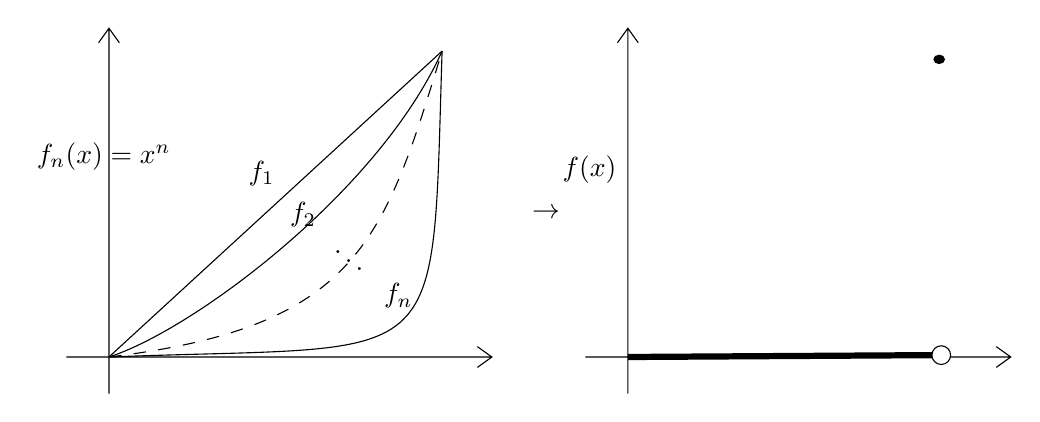
\begin{tikzpicture}[x=0.75pt,y=0.75pt,yscale=-1,xscale=1]
%uncomment if require: \path (0,478); %set diagram left start at 0, and has height of 478

%Shape: Axis 2D [id:dp905814360049316] 
\draw  (72,381.4) -- (277,381.4)(92.5,223) -- (92.5,399) (270,376.4) -- (277,381.4) -- (270,386.4) (87.5,230) -- (92.5,223) -- (97.5,230)  ;
%Shape: Axis 2D [id:dp0627612849597261] 
\draw  (322,381.4) -- (527,381.4)(342.5,223) -- (342.5,399) (520,376.4) -- (527,381.4) -- (520,386.4) (337.5,230) -- (342.5,223) -- (347.5,230)  ;
%Straight Lines [id:da2673655934702972] 
\draw    (92.5,381.4) -- (253,234) ;


%Straight Lines [id:da766634506285276] 
\draw [line width=2.25]    (342.5,381.4) -- (489,380.5) ;


%Shape: Ellipse [id:dp7944840513243177] 
\draw  [fill={rgb, 255:red, 0; green, 0; blue, 0 }  ,fill opacity=1 ] (490,238) .. controls (490,239.1) and (491.12,240) .. (492.5,240) .. controls (493.88,240) and (495,239.1) .. (495,238) .. controls (495,236.9) and (493.88,236) .. (492.5,236) .. controls (491.12,236) and (490,236.9) .. (490,238) -- cycle ;
%Shape: Circle [id:dp9726229856614172] 
\draw  [fill={rgb, 255:red, 255; green, 255; blue, 255 }  ,fill opacity=1 ] (489,380.5) .. controls (489,378.01) and (491.01,376) .. (493.5,376) .. controls (495.99,376) and (498,378.01) .. (498,380.5) .. controls (498,382.99) and (495.99,385) .. (493.5,385) .. controls (491.01,385) and (489,382.99) .. (489,380.5) -- cycle ;
%Curve Lines [id:da8879947029325801] 
\draw    (92.5,381.4) .. controls (134,368) and (223,301) .. (253,234) ;


%Curve Lines [id:da5540476052003762] 
\draw  [dash pattern={on 4.5pt off 4.5pt}]  (92.5,381.4) .. controls (212,367) and (225,326) .. (253,234) ;


%Curve Lines [id:da7987092769906381] 
\draw    (92.5,381.4) .. controls (257,375) and (248,393) .. (253,234) ;





% Text Node
\draw (90,285) node   {$f_{n}( x) =x^{n}$};
% Text Node
\draw (303,312) node   {$\rightarrow $};
% Text Node
\draw (166,293) node   {$f_{1}$};
% Text Node
\draw (186,313) node   {$f_{2}$};
% Text Node
\draw (232,352) node   {$f_{n}$};
% Text Node
\draw (208,331) node   {$\ddots $};
% Text Node
\draw (324,291) node   {$f( x)$};


\end{tikzpicture}
}
    \caption{$f_n$'s are continuous $\forall n$ but their limit is not}
    \label{fig:ptwiseCont}
\end{figure}

\subsection{Point-wise convergence destroys integral:}
Let $f_n(x)=(2n+2)x(1-x^2)^n$ on $[0,1]$ and $f_n(0)=f_n(1)=0$.
\vspace{-1.5in}
\begin{figure}[!ht]
    \centering
    \scalebox{0.6}{


\tikzset{every picture/.style={line width=0.75pt}} %set default line width to 0.75pt        

\begin{tikzpicture}[x=0.75pt,y=0.75pt,yscale=-1,xscale=1]
%uncomment if require: \path (0,478); %set diagram left start at 0, and has height of 478

%Shape: Axis 2D [id:dp5116854562026876] 
\draw  (224,201.4) -- (429,201.4)(244.5,43) -- (244.5,219) (422,196.4) -- (429,201.4) -- (422,206.4) (239.5,50) -- (244.5,43) -- (249.5,50)  ;
%Shape: Axis 2D [id:dp9643251095140839] 
\draw  (445,201.4) -- (650,201.4)(465.5,43) -- (465.5,219) (643,196.4) -- (650,201.4) -- (643,206.4) (460.5,50) -- (465.5,43) -- (470.5,50)  ;
%Curve Lines [id:da26994130810027617] 
\draw    (244.5,201.4) .. controls (261,-4) and (348,198) .. (409,202) ;


%Curve Lines [id:da8291195950058514] 
\draw    (244.5,201.4) .. controls (255,-81) and (297,199) .. (409,202) ;


%Curve Lines [id:da809996449988654] 
\draw    (244.5,201.4) .. controls (259,-190) and (235,193) .. (409,202) ;


%Straight Lines [id:da12190932696161982] 
\draw [line width=2.25]    (625,201) -- (465.5,201.4) ;




% Text Node
\draw (446,98) node   {$\rightarrow $};
% Text Node
\draw (224,70) node   {$f_{n}( x)$};
% Text Node
\draw (448,72) node   {$f( x)$};
% Text Node
\draw (337,126) node   {$f_{1}$};
% Text Node
\draw (293,80) node   {$f_{2}$};
% Text Node
\draw (273,21) node   {$f_{n}$};


\end{tikzpicture}
}
    \caption{$f_n$'s are continuous $\forall n$ but their limit is not}
    \label{fig:ptwiseInt}
\end{figure}

Note from Fig. \ref{fig:ptwiseInt} that $f_n\to 0\implies \int^1_0 f = 0$, but $\int^1_0 f=1$.
Therefore, point-wise convergence does not preserve the value of the integral.

\subsection{Point-wise convergence destroys integrability:}
Let $f_N(x)=1$ if $x=m/n,\,n\leq N$ and $0$ otherwise.
Since $f_N$ has finitely many discontinuities on $[0,1]\implies f_N\in\mathcal{R}$.
However, $\lim_{N\to\infty f_N\to}$ Dirichlet's function, which is not integrable.

Therefore, we need to come up with a better criterion for convergence of sequences of functions that preserve these properties.

\section{Uniform Convergence.}
\begin{definition}[Uniform Convergence]
We say $f_n\to f$ \emph{uniformly} on $E\subset X$ if for any $\varepsilon>0\,\exists N_\varepsilon>0$ such that $\abs{f_n(x)-f(x)}<\varepsilon$ if $n\geq N_\varepsilon$ for \emph{any} $x\in E$.
\end{definition}
\begin{definition}[Uniform norm]
$f_n\to f$ uniformly on $E\iff\sup_E \abs{f_n-f}\to 0$.
Then we can define the uniform norm as $\norm{f_n-f}\coloneqq \sup_E \abs{f_n-f}$.
\end{definition}
In other words, we claim uniform convergence w.r.t. to this newly defined distance approaching zero.

\subsection{Cauchy criterion for Uniform Convergence.}
$f_n$ is a uniformly convergent sequence of functions on $E$ if for any $\varepsilon>0,\exists N_\varepsilon>0$ such that $\abs{f_n(x)-f_m(x)}<\varepsilon$ if $n,m>N_\varepsilon,\,\forall x\in E$.

Similarly, for series convergence, $\sum f_n(x)$ converges uniformly on $E\iff$ for any $\varepsilon>0,\,\exists N_\varepsilon>0$ such that $\abs{\sum^m_{k=n}f_k(x)}\leq \varepsilon$ if $m\geq n\geq N_\varepsilon$. 

\begin{theorem}[Weierstrass M-test]
Suppose $\exists M_n\geq 0$ such that $\sum^\infty_0 M_n$ is finite and $\abs{f_x(x)}\leq M_n,n\geq n_0\,\forall x\in E\implies \sum f_n(x)$ converges uniformly on $E$.
\end{theorem}

\subsection{Uniform convergence \& continuity.}
Let $E\subset X$ and $c$ a limit point of $E$.
Let $f_n:E\to \reals$ and let $A_n=\lim_{x\to c} f_n(x)$ exist.
If $f_n\to f$ uniformly on $E$, then $A=\lim_{x\to c}f(x)$ exists and $A=\lim_{n\to\infty} A_n$, i.e.,
\begin{equation*}
\lim_{n\to\infty} \underbrace{\lim_{x\to c}f_n(x)}_{A_n} = \lim_{x\to c}\underbrace{\lim_{n\to\infty} f_n(x)}_{f(x)}
\end{equation*}
\begin{remark}
This swapping of limits is allowed only for uniform convergence. As we saw in the previous section, point-wise convergence destroys preservation of limits.\\
\emph{Corollary:} If $f_n\to f$ uniformly on $E$ and $f_n$'s are continuous on $E\implies f(x)$ is continuous on $E$.
\end{remark}

\subsection{Uniform convergence \& integrals.}
Let $f_n:[a,b]\to\reals,f_n\in\mathcal{R}(\alpha)$ w.r.t some $\alpha$ on $[a,b]$.
If $f_n\to f$ uniformly on $[a,b]\implies f\in \mathcal{R}(\alpha)$ on $[a,b]$ and 
\begin{equation*}
\int^b_a fd\alpha = \lim_{n\to \infty} \int^b_a f_n d\alpha
\end{equation*}

\subsection{Uniform convergence \& differentiation.}
Suppose $f_n:(a,b)\to\reals$ be differentiable on $(a,b)$ and if $f_n\to f$ uniformly, then 
\begin{equation*}
\lim_{n\to\infty} f'_n(x) = \left(\lim_{n\to\infty}f_n(x)\right)'
\end{equation*}

\section{Equicontinuous Families.}

\section{Stone-Weierstrass theorem.}

\end{document}